\documentclass[11pt]{jsarticle}

\usepackage{amsmath,amsthm,amssymb}
\usepackage[dvipdfmx]{graphicx}
\usepackage{bm}
%
\usepackage{multirow}
\usepackage{wrapfig}
%
\pagestyle{empty}
%% 高さの設定
\setlength{\textheight}{\paperheight}   % ひとまず紙面を本文領域に
\setlength{\topmargin}{-5.4truemm}      % 上の余白を20mm(=1inch-5.4mm)に
\addtolength{\topmargin}{-\headheight}  % 
\addtolength{\topmargin}{-\headsep}     % ヘッダの分だけ本文領域を移動させる
\addtolength{\textheight}{-40truemm}    % 下の余白も20mmに%% 幅の設定
\setlength{\textwidth}{\paperwidth}     % ひとまず紙面を本文領域に
\setlength{\oddsidemargin}{-5.4truemm}  % 左の余白を20mm(=1inch-5.4mm)に
\setlength{\evensidemargin}{-5.4truemm} % 
\addtolength{\textwidth}{-40truemm}     % 右の余白も20mmに

%
\abovecaptionskip=-1pt
%\belowcaptionskip=-1pt
%
\renewcommand{\baselinestretch}{0.95} % 全体の行間調整
\renewcommand{\figurename}{Fig.}
\renewcommand{\tablename}{Tab.}
%
\makeatletter 
\def\section{\@startsection {section}{1}{\z@}{1.5 ex plus 2ex minus -.2ex}{0.5 ex plus .2ex}{\large\bf}}
\def\subsection{\@startsection{subsection}{2}{\z@}{0.2\Cvs \@plus.5\Cdp \@minus.2\Cdp}{0.1\Cvs \@plus.3\Cdp}{\reset@font\normalsize\bfseries}}
\makeatother 
%

\begin{document}

%%%%%%
% はじめに
%%%%%%
\begin{center}
{\Large \textgt{11. MD シミュレーションによるネットワークポリマーのゴム弾性}}
\end{center}

\begin{flushright}
東亞合成 佐々木裕

Tel: 052-611-9923, e-mail: hiroshi\_sasaki$@$mail.toagosei.co.jp
\end{flushright}

\vspace{0.5\baselineskip}
\section{はじめに}

ゴム弾性の古典的なモデルは、ネットワークを構成するストランドをガウス鎖とし、その結節点のミクロな変形がマクロな変形と相似でアフィン変形するとした「ネオ・フッキアンモデル」である。
この古典的なモデルからの発展形として、主として二つの重要な考え方がある。
一つは、結節点の揺らぎに注目したモデルであり、結節点がその平均の位置から自由に揺らぐとした「ファントムネットワークモデル~\cite{James1943}」と呼ばれる。
もう一つが、ストランドに Kuhn らが提唱した「鎖の伸びきり効果」を逆ランジュバン関数で表したモデル~\cite{Kuhn1942} を用い、ランダムに配置された鎖を想定した「フルチェインモデル~\cite{Wu1993}」が提案されている。

ポリマーのMDシミュレーションでは、ポリマー鎖のすり抜けを抑制し絡み合いを表した 「KG 鎖」と呼ばれるビーズ・スプリングモデル~\cite{Kremer1990} が実在鎖との整合性がよいモデルとして広く用いられ、
また、ビーズ間のポテンシャルを省略してポリマー鎖のすり抜けを許容したポリマー鎖は「ファントム鎖」と呼ばれている。
Everaers らは、規則構造を有するネットワークを用いて「KG 鎖」と「ファントム鎖」の比較を行い、各種のゴム弾性理論との高い整合性を報告している~\cite{Everaers1999}。
この検討では規則的なネットワーク構造に起因したノーマルモードがみられ、すり抜けを許容した「ファントム鎖」を用いた場合においてもアフィン変形する「ネオ・フッキアンモデル」としての挙動を示すことが確認されている。

我々は、規則構造ネットワークのユニットセル間における規則性をランダムへと変えてノーマルモードを抑制することで、結節点の揺らぎに由来する「ファントムネットワークモデル」の構築を検討した。

本報告では、平衡構造での鎖の挙動、及び、大変形時の挙動に注目した検討結果について報告する。

\section{シミュレーション}

ランダムな結合性を有するネットワークを作成し、その平衡状態および一軸伸長時の振る舞いについて、OCTA 上の COGNAC シミュレーターを用いた分子動力学シミュレーションにより評価した。

\subsection{ポテンシャルの設定}

KG 鎖は、非結合ポテンシャルとして各ビーズ間に LJ ポテンシャル $U_{LJ}(r)$、ボンドポテンシャルに FENE-LJ ポテンシャル $U_{FENE}(r)$ を用いた。
ファントム鎖は非結合ポテンシャルを省略し、ボンドポテンシャルに FENE-LJ、あるいは、ハーモニックポテンシャル($k=30$)とした。

\vspace{1mm}
\begin{figure}[hb]
\begin{minipage}{0.33\hsize}
	\begin{center}
	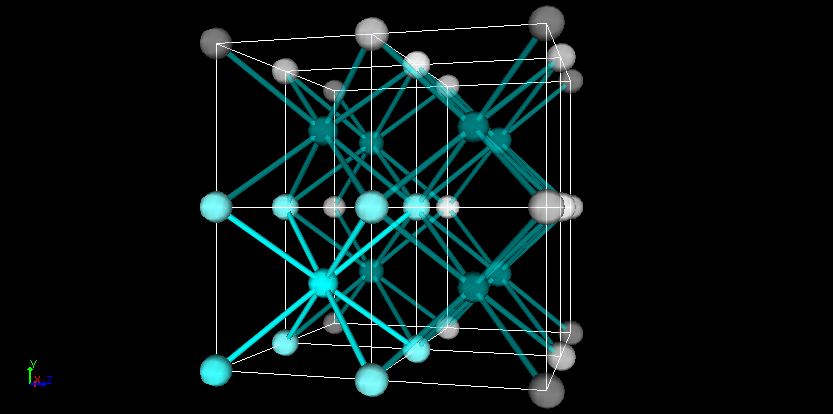
\includegraphics[width=50mm]{./fig/8_per.png}
	\caption{2x2x2 Cells of 8 strands}
	\label{fig:cells}
	\end{center}
\end{minipage}
\begin{minipage}{0.33\hsize}
	\begin{center}
	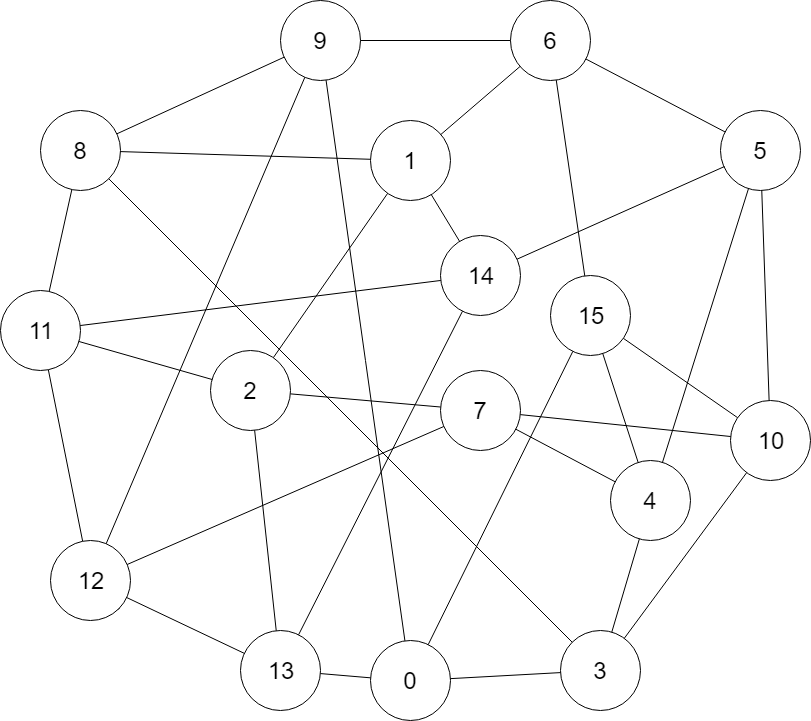
\includegraphics[width=30mm]{./fig/Network.png}
	\caption{Topological NW model}
	\label{fig:topo}
	\end{center}
\end{minipage}
\begin{minipage}{0.33\hsize}
	\begin{center}
	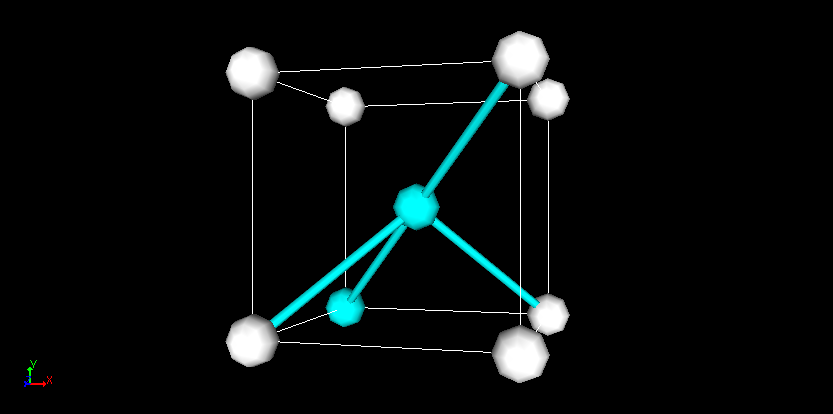
\includegraphics[width=50mm]{./fig/8_4.png}
	\caption{Reduced to 4 starands}
	\label{fig:red4}
	\end{center}
\end{minipage}
\end{figure}
\vspace{-3mm}

\subsection{ネットワークモデルの作成}
体心立方構造の各格子点をN 個のビーズからなるストランドでつないだ「八本鎖モデル」のユニットセルを作成し、その連なりとしてネットワークの初期構造を表した(Fig. \ref{fig:cells})。
任意の分岐数$f$($f=3\sim6$)となるように、以下のアルゴリズムで各ノードの隣接関係にランダム性を導入した。
\vspace{-2mm}
\begin{enumerate}
\item
実空間で初期構造(ストランドの末端間距離をメルトと同一と設定)の作成(Fig. \ref{fig:cells})。
\item
初期構造に対応したトポロジーモデルを用いてノードごとのエッジ数(分岐数)に変換(Fig. \ref{fig:topo})。
\item
そのトポロジーモデルに対応するように、実空間の初期構造からストランドを除去(Fig. \ref{fig:red4})。
\item
任意の密度とするため、複数のネットワークが相互貫入した IPN 構造の多重度(Multi)を設定。
\end{enumerate}
\vspace{-4mm}

\section{結果と考察}

ここでは、ボンドポテンシャルとしてハーモニックポテンシャルを用いたファントム鎖ストランドを用いた三分岐モデル($f=3$)の結果についてまとめた。
\subsection{ストランドの末端間距離 $\langle \bm{R} \rangle$ の分布関数}

ストランド(セグメント数 N=20 )の末端間距離の分布関数を Fig. \ref{fig:e2e} に示した。メルトポリマー鎖と比較して若干末端間距離が伸びていた(平均で比較して数 \% 程度)が、分布関数の形状はほぼ再現できた。

\subsection{一軸伸長}
ファントムネットワークでは、バルク内部の架橋点の揺らぎのために伸長によるストランドのエントロピー変化が減少しバルクとしての弾性率が低下するとされている~\cite{James1943}。

この減少率を$F_P$と書くとこの値はシステムサイズ依存性があり、それぞれの極限で、
\vspace{-2mm}
\begin{align}
&\begin{cases}
F_P^{large}=1-\dfrac{2}{f}\;\;\;\text{十分に大きなシステム} \\[10pt]
F_P^{min} \simeq \dfrac{f-1}{f+1}\;\;\;\text{最小限のシステム} 
\end{cases}\\
&\sigma_{nom.}=F_P \times \nu k_BT \left( \lambda-\dfrac{1}{\lambda^2} \right)
\end{align}

システム一辺当たりのユニットセル数が異なるシステム(Cell-1d=3$\sim$6)を一軸伸長($10^{-4}\lambda/\tau$)した時の SS カーブを Fig. \ref{fig:SS_cells} に示した。Cell-1d=3と小さいシステムサイズでは、$F_P^{min}$($\simeq$ 0.5 for 3-Chain) に対応した Quasi P. の曲線にほぼ重なっていたが、セル数の増加により、$F_P^{large}$($\simeq$ 0.33 for 3-Chain) であらわされる Phantom へと漸近し、Cell-1d=5 では$F_P\simeq0.4$程度となっていることが確認できた。

%\subsection{伸びきり効果}
%
%以下のフルチェインモデルでの伸びきり効果~\cite{Wu1993}の表式に、Cell-1d=5 で$F_P\simeq0.4$となることをセグメント数 $N$: $20\rightarrow60$ として考慮すると、 大きな変形まで良い一致を示した(Fig. \ref{fig:stretch})。
%\vspace{-2mm}
%\begin{align}
%&\sigma_{Full} = E \dfrac{\sqrt{N}}{4\pi} \int_0^{\pi} \int_0^{2\pi} \mathcal{L}^{-1} \left( \dfrac{\lambda}{\sqrt{N}} \right) \dfrac{\lambda_i^2 m_i^2}{\lambda} \sin \theta \mathrm{d} \theta \mathrm{d} \phi \\
%\text{where}\;\;&m_0 = \sin \theta \cos \theta,\; m_1 = \sin \theta \sin \phi, \; m_2 = \cos \theta,\;\lambda^2 = \sum_{i=0}^2 \lambda_i^2m_i^2 \notag
%\end{align}
%\normalsize

\vspace{-3mm}

\begin{figure}[hb]
\begin{minipage}{0.5\hsize}
	\begin{center}
	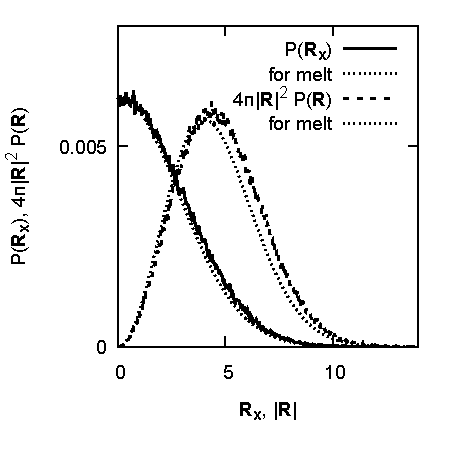
\includegraphics[width=65mm]{./fig/PR_BW.pdf}
	\caption{End to end distance of strands for 3-Chain model(N20, Cell-1d=5, Multi=4)}
	\label{fig:e2e}
	\end{center}
\end{minipage}
\begin{minipage}{0.5\hsize}
	\begin{center}
	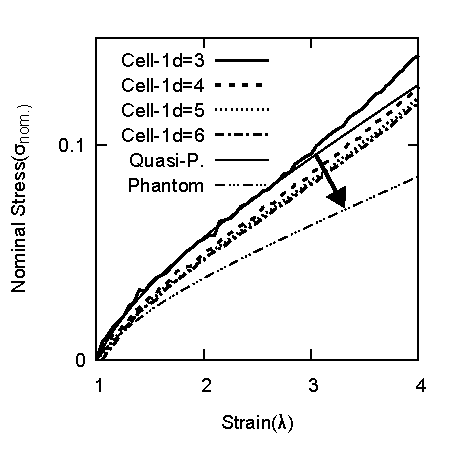
\includegraphics[width=65mm]{./fig/SS_all_BW.pdf}
	\caption{SS Curves for 3-Chain model(N20) with varied number of Cells}
	\label{fig:SS_cells}
	\end{center}
\end{minipage}
%\begin{minipage}{0.33\hsize}
%	\begin{center}
%	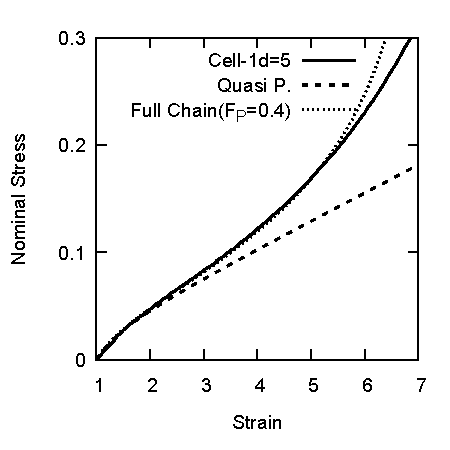
\includegraphics[width=50mm]{./fig/Stretch_BW}
%	\caption{Stretched effect for 3-Chain model(N20) Cell-1d=5}
%	\label{fig:stretch}
%	\end{center}
%\end{minipage}
\end{figure}
\vspace{-3mm}


\bibliographystyle{achemso}
%{elsart-num}
%{junsrt-2}
\bibliography{./library.bib}

\end{document}